\documentclass[12pt, letterpaper, twoside]{article}
\usepackage[utf8]{inputenc}
\usepackage{graphicx}
\begin{document}
\title{IN2090 Oblig1}
\author{Espen Lønes}
\date{\today}
\maketitle
\ \\
Oppgave 1)\\
\ \\
Et ping tuppel kan relatere til flere tuppler i Pong (1:N), via zip.\ Men det kan også ikke relatere til noen tuppler i Pong i det hele tatt (ikke total deltagelse).\\
Et tuppel i Pong må relatere til nøyaktig ett tuppel i Ping via Zip (total deltagelse og 1:N).\\
\newpage
\ \\
Oppgave 2)\\
\ \\
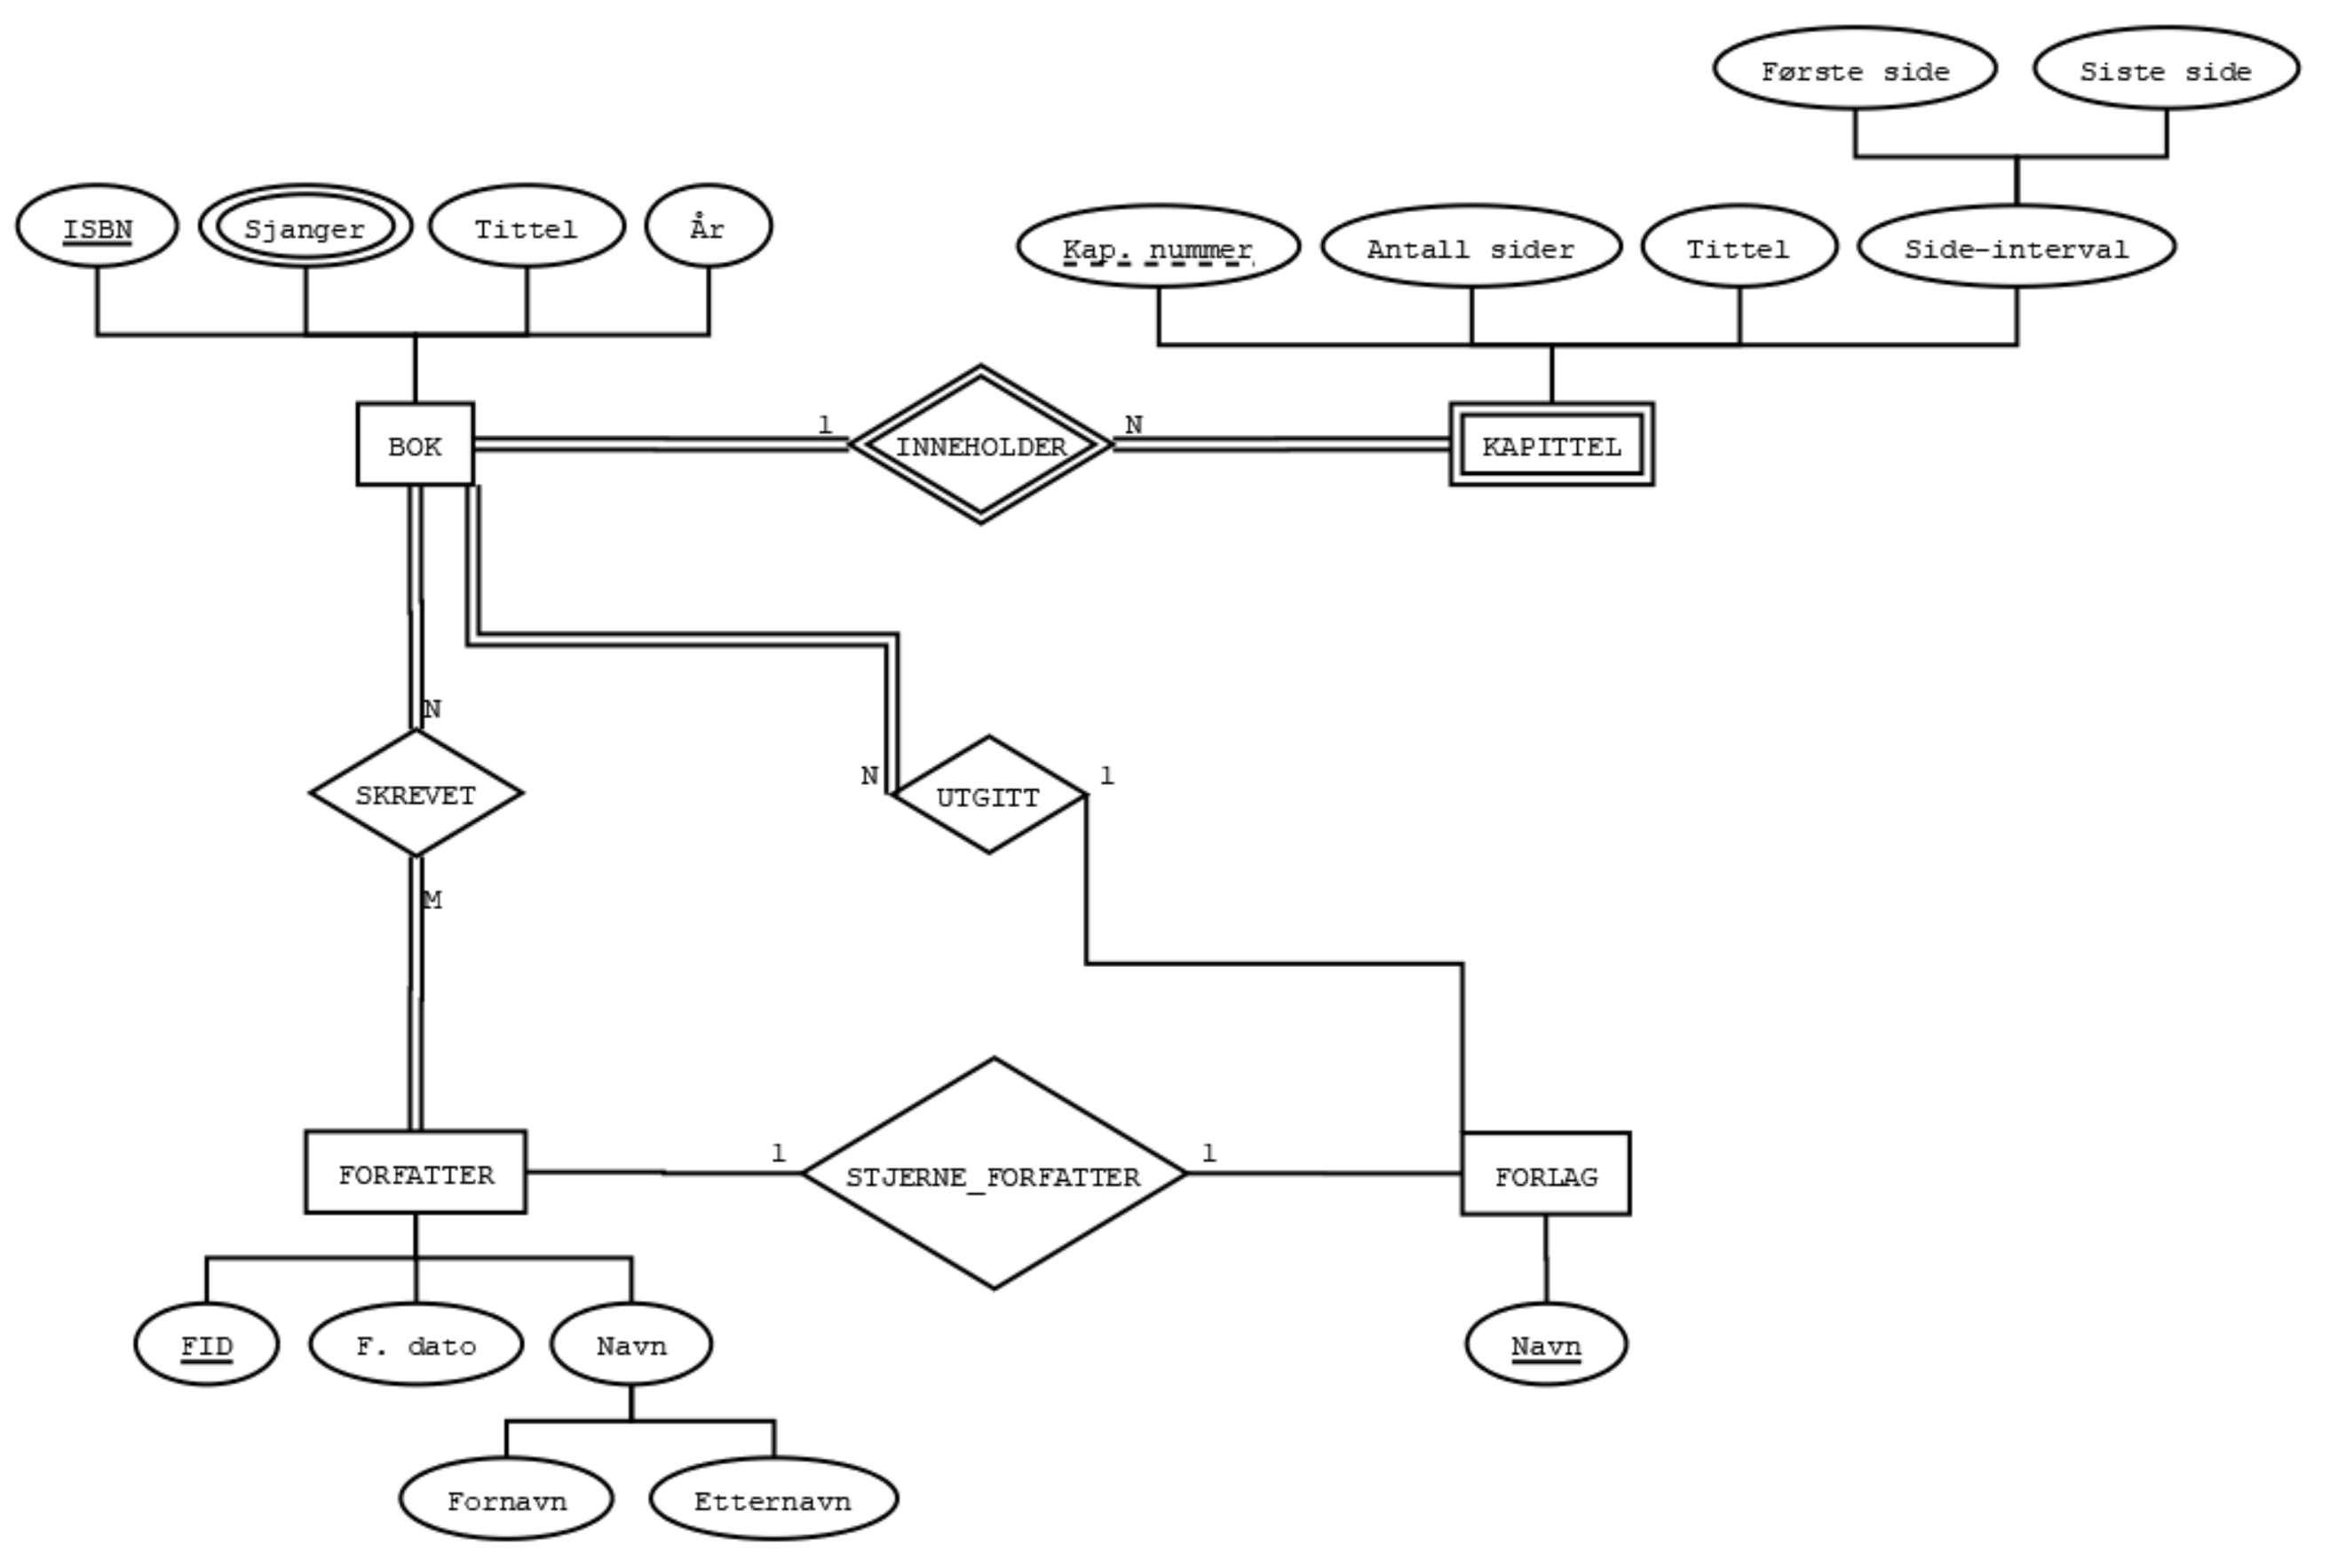
\includegraphics[scale=0.5]{Oppgave2.png}\\
\ \\
Velger å ikke ha total deltagelse fra forlag til bok, siden jeg mener det kan finnes nye forlag som ikke har gitt ut bøker ennå.\\
Velger også å ha total deltagelse fra forfatter til bok, siden man er ikke en forfatter om man ikke har skrevet minst en bok.
\newpage
\ \\
Oppgave 3)\ \\
\ \\
Person(\underline{Personnr.}, Navn, Gate, Gatenr., Postnr.)
\ \\
Hus(\underline{Gate, Gatenr., Postnr.}, Ant. Etasjer, Areal)
\ \\
Telefonnr.(\underline{Personnr., Nummer})
\ \\
\ \\
\ \\
Fremmednøkler:\\
\ \\
Person(Gate, Gatenr., Postnr.) er fremmednøkkel $\rightarrow$ \\
Hus(Gate, Gatenr., Postnr.). For å representere BOR\_I relasjonen.
\ \\
\ \\
Telefonnr.(Personnr.) er fremmednøkkel $\rightarrow$ Person(Personnr.)
\end{document}